\documentclass{article}
\usepackage{../common/kurzinfo}
%\usepackage{lmodern}
%\newfont{\klitzeklein}{cmss10 at 8.5pt}

\newcommand{\frage}[1]{\vspace*{1ex}

\textbf{#1}\\
}

\renewenvironment{artikel}[1]{

\noindent
  \begin{minipage}[t]{\linewidth}
    \begin{large} 
      \setlength{\baselineskip}{2ex}
      \textbf{#1}\\[-3ex]
    
\end{large}
\sloppy
\vspace{2mm}
  }{
  \end{minipage}
\vspace*{4mm}
}

\verantwortlich{M. Nick} % HIER VISDP EINTRAGEN
\druck{AStA Druckerei}
\auflage{ca. 500} %HIER APPROXIMIERTE AUFLAGE EINTRAGEN
%\ausgabennummer{168} %% BITTE NACHSEHEN
\begin{document}
%<doppelseite>
%% DATUM KORRIGIEREN !!!%%%%

\begin{vorderseite}{Stand 18. November 2013}{Prüfungsrecht} %erste Seite, Datum und Ueberschrift
\zweispalten{.5\linewidth}
{%Kommentar: linke Spalte 

%Texte einbinden
\vspace{-3.0ex}
\begin{artikel}{Wohnungssuche}
Um das Leben in Aachen genie�en zu k�nnen, willst Du nat�rlich eine geniale
Wohnung Dein eigen nennen. Nat�rlich hast Du Dir Deine Traumwohnung im Kopf
schon entworfen und eingerichtet, doch leider ist sie in dieser Form noch
nicht gebaut worden. In diesem Text findest Du deshalb ein paar Tips, wie
Du an eine Wohnung kommen kannst, die m�glichst viele Deiner W�nsche erf�llt.
\end{artikel}

\begin{artikel}{Ansprechpartner}
Erste Ansprechpartner bei Fragen zu Prüfungen sind die Fachschaften und der AStA. Wende Dich frühzeitig bei Fragen und Problemen an Deine dortigen Vertreterinnen und Vertreter. Fachschaften und AStA bieten regelmäßig Sprechstunden an und sind per Mail erreichbar. Die zuständigen Menschen im AStA erreicht ihr unter \email{pruefungsrecht@asta.rwth-aachen.de}.
\end{artikel}

\begin{artikel}{Rechtsanwalt für Prüfungsrecht im AStA}
Neben einer Rechtsberatung für allgemeine Rechtsfragen bietet der AStA donnerstags vierzehntägig eine besondere Rechtsberatung für Prüfungsrechtsfragen an. Die Beratung wird durchgeführt von der Kanzlei Birnbaum aus Köln, die sich auf Prüfungs- und Hochschulrecht spezialisiert hat. Termine werden nur persönlich im AStA gegen eine Kaution von zehn Euro vergeben.
\end{artikel}

\begin{artikel}{Deine Prüfungsordnung}
Hochschulprüfungen werden aufgrund von Prüfungsordnungen abgelegt. Das sind Satzungen, die Vorgaben durch Gesetze, Grundrechte und Rechtsprechung unterliegen. Zunächst ist wichtig, dass du deine Prüfungsordnung gelesen hast. Deine aktuell gültige Prüfungsordnung findest du auf der Homepage deiner Fakultät und online in den Amtlichen Bekanntmachungen der RWTH. Achte auch auf Änderungsordnungen. Prüfungsordnungen legen u.a. die abzulegenden Prüfungsleistungen, ihre Art und Dauer fest, ebenso die Möglichkeiten der An- und Abmeldung und Wiederholungsmöglichkeiten.
2009 hat der Senat der RWTH Rahmenprüfungsordnungen für alle Bachelor- und Masterstudiengänge erlassen, um die Bedingungen für alle Studierenden vergleichbar zu machen. Genauere Informationen findest du im Kurzinfo zu den RahmenPO.


\end{artikel}

%\begin{artikel}{Rahmenprüfungsordnungen}
\end{artikel}

\begin{artikel}{\Large Prüfungsanfechtung}\end{artikel}
\vspace{-3ex}
\begin{artikel}{Kausalität}
Im Allgemeinen kann eine Prüfungsentscheidung aufgehoben werden, wenn gegen Verfahrensvorschriften verstoßen wurde. Wurde also ein Fehler bei Deinem Prüfungsverfahren gemacht, kann dies ein Anrecht darauf begründen, die Prüfung zu wiederholen. Das gilt aber aber nur, wenn ein Einfluss des Verfahrensfehlers auf das Ergebnis nicht ausgeschlossen werden kann. Hättest Du zum Beispiel eine Prüfung auch dann nicht bestanden, wenn Du bei einer fehlerhaft gestellten Aufgabe alle Punkte erreicht hättest, so kann der Fehler keine Auswirkung auf Dein Bestehen gehabt haben.

Die Beweislast dafür, dass ein Verfahrensfehler keine Auswirkungen hatte, liegt in der Regel bei der Prüfungsbehörde.
\end{artikel}


}
{%Kommentar: rechte Spalte
\begin{artikel}{Verwaltungsinternes Überdenken}
Der Prüferin bzw. dem Prüfer steht ein gewisser Beurteilungsspielraum zu, innerhalb dessen eine gerichtliche Überprüfung nicht möglich ist.

Aus diesem Grund gibt es das verwaltungsinterne Überdenkungsverfahren, bei dem du der Prüferin bzw. dem Prüfer anhand von konkreten Einwänden die Möglichkeit geben musst, die Prüfungsentscheidung zu überdenken - in der Regel im Rahmen der Einsicht in die Prüfungsakten. Eine Verschlechterung ist ausgeschlossen, es werden nur die beanstandeten Einzelwertungen überprüft.
\end{artikel}

\begin{artikel}{Widerspruchsverfahren}
Prüfungsentscheidungen sind Verwaltungsakte. Wichtigstes Rechtsmittel gegen sie ist der Widerspruch. Mit diesem wendest Du dich an die zuständige Widerspruchsbehörde, in der Regel an Deinen Prüfungsausschuss. Der Widerspruch muss schriftlich und begründet erfolgen. In der Regel beträgt die Frist hierfür einen Monat. Sie verlängert sich auf ein Jahr, wenn keine oder eine fehlerhafte Rechtsbehelfsbelehrung erfolgt ist. Der Prüfungsausschuss entscheidet zeitnah über den Widerspruch. Wenn Dein Widerspruch nicht erfolgreich ist, kannst Du Anfechtungsklage vor dem Verwaltungsgericht erheben. Wenn Du nicht weißt, wie oder an wen Du Deinen Widerspruch richten musst, hilft Dir Deine Fachschaft oder der AStA.
\end{artikel}

\begin{artikel}{Klageverfahren}
Vor Gericht kann neben fachlichen Fragen nur geprüft werden, ob z.B. das Prüfungsverfahren mit erheblichen Fehlern belastet ist, allgemeingültige Bewertungsgrundsätze nicht beachtet wurden oder Willkür vorliegt. Ein Gerichtsverfahren vor dem Verwaltungsgericht dauert meist ein bis zwei Jahre. Vor allem wenn eine Prüfung endgültig nicht bestanden wurde, wird daher gleichzeitig ein Verfahren auf Erlass einer einstweiligen Anordnung angestrebt, damit du dein Studium erst einmal fortsetzen kannst.
\end{artikel}

\begin{artikel}{Kosten}
Beim Widerspruchsverfahren entstehen normalerweise nur Kosten, wenn anwaltliche Hilfe in Anspruch genommen wird. Die Kosten für eine Anfechtungsklage und das Eilverfahren werden im Wesentlichen durch die Anwaltskosten bestimmt, die vom gewählten Rechtsanwalt, Streitwert, Aufwand etc. abhängen. Normalerweise ist auch die Beratung kostenpflichtig, eine kostenlose Beratung für alle Studierenden der RWTH gibt es regelmäßig im AStA.

Beachte, dass eine möglicherweise vorhandene Rechtsschutzversicherung unter Umständen Verwaltungsrecht und insbesondere Prüfungsrecht nicht abdeckt.
\end{artikel}

\begin{artikel}{Folgen}
Bei einer erfolgreichen Prüfungsanfechtung wird das Gericht festlegen, wie ein festgestellter Mangel zu beseitigen ist. In den meisten Fällen ist die Prüfung zu wiederholen. Bei erfolgreicher Prüfungsanfechtung gilt diese Entscheidung grundsätzlich nur für Dich.
\end{artikel}

}

\vspace*{-2cm}
\end{vorderseite}

%<zweiterparameter>
\begin{rueckseite}{Stand 18. November 2013}{Prüfungsrecht} %Rueckseite, dass die immer so hei"st wie die Vorderseite, habe ich (noch) nicht hingekriegt.
\zweispalten{.425\linewidth}%Breite der linken Spalte, der Kontaktblock sitzt im Stylefile\ldots
{
\begin{artikel}{FAQ Krankheit, Rücktritt und Versäumnis}
Die Möglichkeiten zum Prüfungsrücktritt werden durch die Prüfungsordnung geregelt. Die meisten Ordnungen ermöglichen neben einer ein- oder mehrmaligen Prüfungsabmeldung den Prüfungsrücktritt aus wichtigem Grund. Der häufigste Grund ist die Prüfungsunfähigkeit wegen Krankheit. Diese muss in der Regel vor Beginn der Prüfung angezeigt werden und die Prüfung darf nicht angetreten werden. Es ist nicht zulässig, mit dem Attest in der Tasche zur Prüfung zu gehen und sich hinterher auf Prüfungsunfähigkeit zu berufen.
Wichtig ist, dass ein Rücktritt von einer Prüfung erklärt, also bekannt gegeben, wird. Wenn du einfach nicht zur Prüfung erscheinst, wird die Prüfung grundsätzlich als "`nicht ausreichend"' gewertet.
Es gibt in Einzelfällen die Möglichkeit, dass Du Deine Prüfungsunfähigkeit erst während oder gar nach der Prüfung feststellst. In diesen Fällen gelten weitergehende Anforderungen an das Attest. Näheres hierzu findest du im "'Wiki Intern"`.
\end{artikel}

\begin{artikel}{FAQ Äußere Prüfungsbedingungen, Prüfungsdauer und Rügepflicht}
Die äußeren Prüfungsbedingungen müssen aus Gründen der Chancengleichheit für alle Prüflinge identisch sein. Gelegentlich treten im Prüfungsablauf aber auch Störungen auf, wie z.B. Lärm, Hitze, Kälte oder beißender Geruch. Überschreiten diese Störung eine Erheblichkeitsschwelle, können sie dein Leistungsvermögen beeinträchtigen.

Dies kannst du nach der Prüfung nur geltend machen, wenn du es unverzüglich bei der Aufsicht oder der Prüferin bzw. dem Prüfer rügst und um Abhilfe bittest. Die Rüge solltest du im Protokoll festhalten lassen. Wenn sofortige Abhilfe nicht möglich ist, kann eine Schreibzeitverlängerung gewährt werden.

Die Prüfungsdauer wird in der Regel durch die Prüfungsordnung bestimmt und muss abgesehen vom Fall der Schreibzeitverlängerung eingehalten werden. Die Prüferin bzw. der Prüfer darf diese weder verkürzen noch verlängern, auch nicht wenn du zustimmst.
\end{artikel}

\begin{artikel}{FAQ Einsichtnahme}
Nach jeder vollständig abgelegten Prüfung steht dir das Recht auf Einsichtnahme in die Prüfungsakten zu, unabhängig davon, ob du eine Prüfung bestanden hast oder nicht. Du musst die Bewertung nachvollziehen können. Die Einsicht nur unter Aufsicht zu erlauben, ist zulässig. Auf jeden Fall muss man dir ausreichend Zeit und Platz zur Verfügung zu stellen. Obwohl dies häufig verweigert wird, hast du das Recht, dir Notizen zu machen und Auszüge zu fertigen. Es muss zur Begründung eines Widerspruchs sogar ermöglicht werden, Kopien anzufertigen oder anfertigen zu lassen, Kosten dafür hast du selbst zu tragen.
\end{artikel}

}
{
\begin{artikel}{FAQ Wiederholungsprüfungen und letzter Versuch}
Die meisten Prüfungsordnungen sehen eine zweimalige Wiederholungsmöglichkeit jeder nicht bestandenen Prüfung sowie eine mündliche Ergänzungsprüfung vor. Wiederholungsprüfungen müssen dabei nicht zwangsläufig nach denselben Verfahrensregeln wie die erste Prüfung durchgeführt werden.

Wenn Du eine oder mehrere Prüfungen nicht bestanden hast und den Studiengang oder die Hochschule wechseln möchtest, können sich Schwierigkeiten ergeben. Lass Dich in so einem Fall beraten.

Leistungen in Prüfungen, mit denen ein Studiengang abgeschlossen wird oder bei deren endgültigen Nichtbestehen keine Ausgleichsmöglichkeit vorgesehen ist, sind von mindestens zwei Prüferinnen oder Prüfern zu bewerten. Nach gängiger Rechtsprechung darf die Zweitkorrektur aber in Kenntnis der Erstkorrektur und -bewertung vorgenommen werden und dabei die Erstkorrektur bestätigt werden.

Ein Sonderfall ist die Bewertung von Aufgaben im Antwort-Wahl-Verfahren (Multiple-Choice). Das Zusammenzählen der Punkte ist keine Bewertung. Die Prüfertätigkeit ist auf das Stellen der Aufgaben vorverlagert. Daher müssen nach aktueller Rechtsprechung bei der Erstellung der Aufgaben zwei Prüferinnen bzw. Prüfer zusammenwirken.
\end{artikel}

\begin{artikel}{FAQ Multiple Choice}
Das Antwort-Wahl-Verfahren, häufig Multiple-Choice genannt, ist rechtlich besonders umstritten. Gemeint sind Aufgaben, bei denen aus vorgegebenen Antwortmöglichkeiten richtige Antworten ausgewählt werden müssen. Dabei gibt es die unterschiedlichsten Formen und Bewertungsarten. Das Verfahren ist zwar einfach in der Auswertung, dafür fehlt aber die Möglichkeit, sinnvoll mit fehlerhaften oder mehrdeutigen Fragestellungen umzugehen. Die Bewertung kann keine Rücksicht auf die Richtigkeit von Antworten nehmen, die von der Erwartung der Prüferin oder des Prüfers abweichen. Daher gibt es hohe Anforderungen an das Stellen der Aufgaben.

%vgl. OVG NRW, AZ 14 B 1109/11: Die Bewertung richtig beantworteter Prüfungsfragen darf nicht deshalb schlechter ausfallen, weil andere Fragen statt gar nicht falsch beantwortet wurden. Damit wird nicht der Wissenstand des Prüflings, sondern allenfalls seine Risikobereitschaft zum Raten beurteilt. Dieser Bewertungsmangel ist allerdings nicht ursächlich geworden, da auch bei Wegfall der Malus-Punkte die Prüfung nicht bestanden ist.

Der Abzug von Punkten für falsch angekreuzte oder fehlerhaft nicht angekreuzte Antworten ist nach neuester Rechtssprechung im Allgemeinen rechtswidrig, da so darüber hinweggetäuscht wird, dass richtige Antworten gewusst wurden. Das bedeutet aber nicht, dass es genügt, alle Antwortmöglichkeiten anzukreuzen. Es darf lediglich für eine falsch beantwortete Aufgabe insgsamt keinen Abzug von Punkten geben.

%vgl bspw. Master-RPO § 9 (2), (3) 
Bei Aufgaben im Antwort-Wahl-Verfahren muss es immer eine relative Bestehensgrenze geben, d.h. die Gesamtleistung aller Teilnehmenden an einer Prüfung muss berücksichtigt werden. Insbesondere ist eine Prüfung im Antwort-Wahl-Verfahren immer als bestanden zu bewerten, wenn 60\,\% der richtigen Antworten gegeben worden sind oder wenn die Anzahl der korrekt gegebenen Antworten höchstens 22\,\% unter dem Durchschnitt derer liegt, die zum ersten Mal an der Prüfung teilnehmen.
\end{artikel}



% IMPRESSUM UND CO.
\fcolorbox{black}{light}{%use white for red style sheet
\begin{minipage}[b]{0.5\textwidth}
\parbox{\linewidth}{
\parbox[t]{.49\linewidth}{
\scriptsize %SCHRIFTGFRÖßE FÜR IMPRESSUM

\textbf{\footnotesize Kontakt zum AStA}\\
Allgemeiner Studierendenausschuss \\
der RWTH Aachen\\
Peterstr. 44-46, 52062 Aachen\\
Tel.: 0241 / 80 - 93792 \\
Fax.: 0241 / 80 - 92394 \\ \\
\url{http://www.asta.rwth-aachen.de/}\\
\email{asta@asta.rwth-aachen.de} \\
\rule{2\linewidth}{.5pt}
\\
}
\parbox[t]{.49\linewidth}{

\scriptsize
\textbf{\footnotesize \"Offnungszeiten}\\
Mo. -- Fr. \hfill{} 10\Uhr{} -- 14\Uhr{} Uhr\hspace*{1ex}\\
\vspace*{0.2ex}

\textbf{\footnotesize{Beratungs- und Servicezeiten}}\\
siehe Homepage\\

\textbf{\footnotesize AStA Sitzungen}\\
\scriptsize Fr. 14\Uhr{} Uhr (natürlich öffentlich!)\\

}

\vspace*{-1ex}

}





\footnotesize{\textbf{Impressum:} AStA der RWTH Aachen, Peterstra"se 44-46, 52062 Aachen}\\
\footnotesize{\textbf{ViSdP:} Johanna Sch"ope, \email{oeffentlichkeit@asta.rwth-aachen.de}}
	

\end{minipage}
}%fcolorbox endet hier
}

\vspace{3ex}
\fcolorbox{black}{light}{\parbox{\linewidth}{\textbf{Haftungsausschluss}%Beispielbox

{\footnotesize Verbindliche Auskünfte erteilen die jeweils zuständigen Stellen. AStA und Redaktion haften nicht für die Inhalte dieses Informationsblattes.}}}
%\begin{artikel}{Linkliste/Weitere Informationen}
\parbox{.1\linewidth}{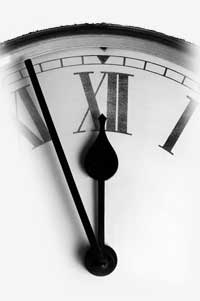
\includegraphics[width=\linewidth]{bilder/uhr}}
\parbox{.9\linewidth}{
\begin{aufzaehlung}
\item \url{www.asta.rwth-aachen.de} -- Webseiten des AStA mit aktuellen Infos und Sprechzeiten der BAf"oG-Beratung
\item \url{www.bafoeg.bmbf.de} -- Bundesministerium f�r Bildung und Forschung, Informationen und BAf"oG-Rechner
\item \url{www.studentenwerk-aachen.de} -- BAf"oG-Amt Aachen
\item \url{www.studis-online.de} und \url{www.bafoegrechner.de} -- aktuelle Infos rund ums BAf"oG
\end{aufzaehlung}}
\vspace*{1ex}

Der AStA bietet auch eine pers"onliche Beratung an. Die genauen Termine findest Du in der unten stehenden Kontaktbox oder auf unserer Webseite unter \url{www.asta.rwth-aachen.de/beratung}. Eine vorherige Terminabsprache ist nicht notwendig. Die Beratung ist kostenlos und erfolgt selbstverst"andlich vertraulich.
\end{artikel}

\end{rueckseite}
%<geschweifteKlammer>
\end{document}  


